\section{La pubblicità}

Questo aspetto è sicuramente importantissimo per la navigazione e l'usabilità. È perfettamente comprensibile che un sito web tragga dei profitti dal proprio lavoro, ed in questo caso essi provengono in primis dalla pubblicità. C'è però modo e modo di gestirla. Gli utenti nella quasi totalità dei casi odiano la pubblicità e chiaramente vorrebbero farne a meno. Esistono plugin per i diversi browser che bloccano le pubblicità ma non cancellano definitivamente il problema.

\subsection{Pubblicità sul layout}

Ora ho disattivato il mio adblocker su firefox e il risultato sono queste aggiunte:

\begin{figure}[H]
\centering

\includegraphics[width=100mm]{images/adv1.png}
\caption{Pubblicità sotto il menu di navigazione}
\end{figure}

\begin{figure}[H]
\centering

\includegraphics[width=100mm]{images/adv2.png}
\caption{Pubblicità in mezzo al menu}
\end{figure}

\begin{figure}[H]
\centering
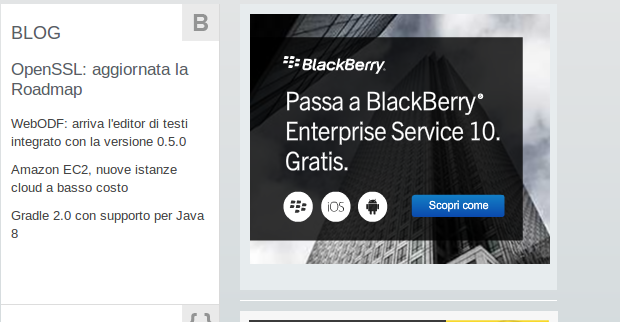
\includegraphics[width=100mm]{images/adv3.png}
\caption{Pubblicità sulla barra laterale}
\end{figure}

Niente di così grave per il momento, in ogni caso più un meno lungo l'intera pagina compaiono pubblicità di ogni tipo, non necessariamente legate al mondo dell'informatica. Questo ancora non è fastidioso ed è sopportabile dall'utente. Una cosa leggermente più vistosa è quando la pubblcità compare sullo sfondo del sito, come in questo caso:

\begin{figure}[H]
\centering

\includegraphics[width=120mm]{images/adv6.png}
\caption{Pubblicità sullo sfondo}
\end{figure}

Come si può notare distoglie chiaramente l'attenzione e provoca frustrazione all'utente.

\subsection{Pop-up}

Una cosa peggiore arriva nel momento in cui cerco di accedere ad un'articolo o una guida. Il risultato è il seguente:

\begin{figure}[H]
\centering
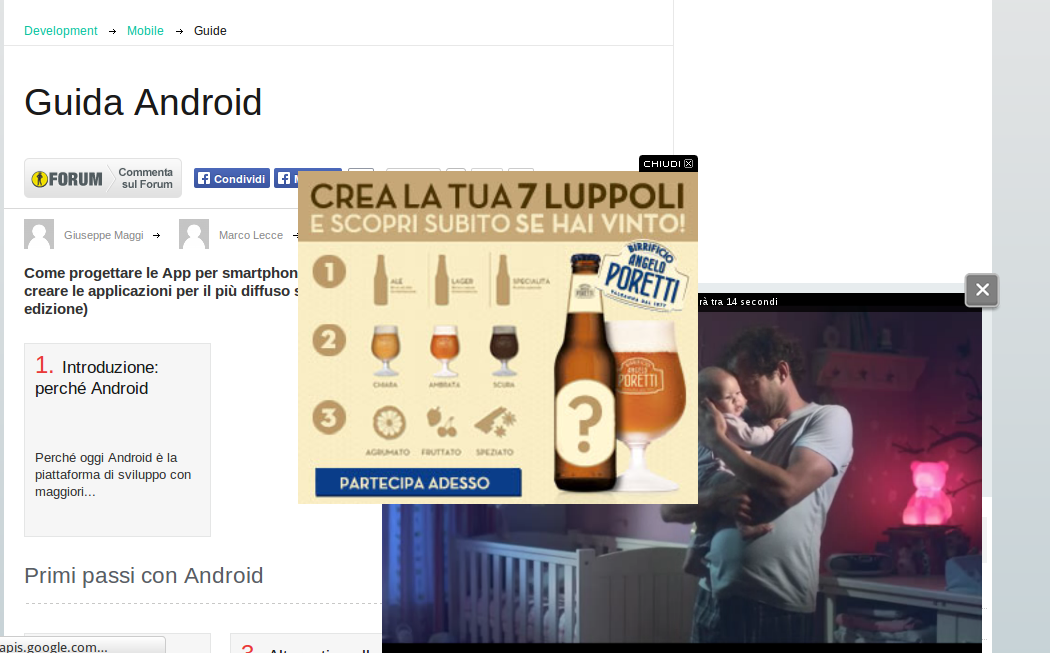
\includegraphics[width=120mm]{images/adv4.png}
\caption{Pop-up all'apertura di un'articolo}
\end{figure}

Come si può notare è apparso un fastidiosissimo pop-up che blocca completamente la lettura e costringe l'utente a chiuderlo. Se l'utente sbaglia a cliccare il pulsante di chiusura rischia chiaramente di essere reindirizzato ad un altro sito. Questa è decisamente una mazzata per l'usabilità, fa passare la voglia a qualunque utente di rimanere nel sito.

\subsection{Video}

Il peggio purtroppo non è ancora arrivato. Se noi abilmente chiudiamo il pop-up sotto possiamo ammirare un bellissimo video (non richiesto) che invade il contenuto della pagina e che parte tranquillamente in automatico anche con il volume.


\begin{figure}[H]
\centering
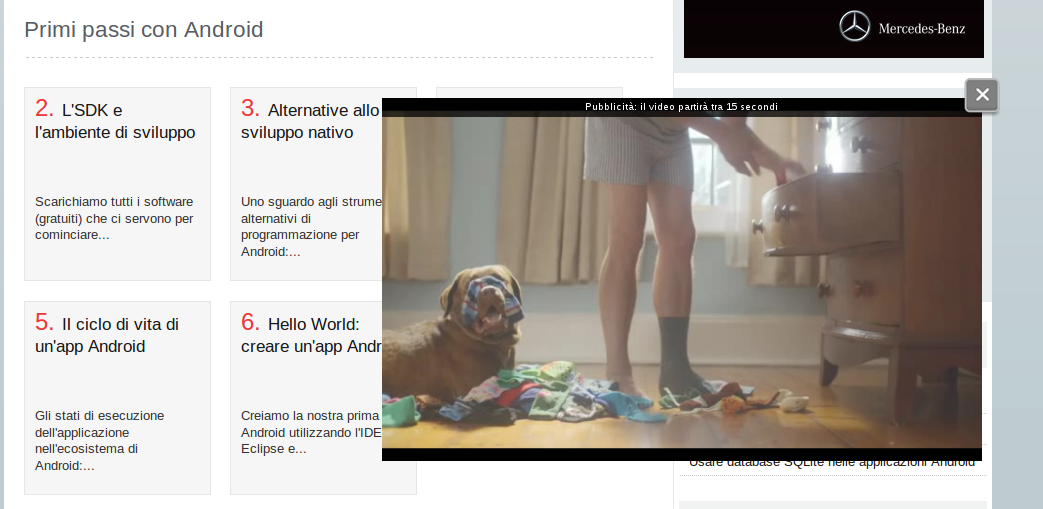
\includegraphics[width=120mm]{images/adv5.png}
\caption{Video di pubblicità invadente}
\end{figure}

Questa è una combo micidiale per l'usabilità, è probabilemente ancora peggio della finestra pop-up precedente. Noterete inoltre come sia incredibilmente ostico mettere il video in pausa.
\linebreak
\linebreak
Tutto questo avviene lungo l'intera navigazione e per ciascuna lezione c'è il video di pubblicità che per la nostra felicità compare ogni volta e disturba la nostra lettura. Questo comporta uno stress notevole da parte dell'utente e una sua diffidenza. Personalmente io evito tutto questo con un adblocker ma un utente normale in questa situazione si ritroverebbe sommerso da pubblcità invadente e fuori contesto senza suo malgrado poter porre rimedio.
\linebreak
\linebreak
In conclusione, la pubblicità è lecita e comprensibile ma questo sito la gestisce in modo pessimo ammazzando letteralmente l'usabilità. Questo aspetto fa precipitare l'intero giudizio del sito, fin qui tutto sommato buono.
